\section{Auswertung}
\label{sec:Auswertung}

%\begin{figure}
%  \centering
%  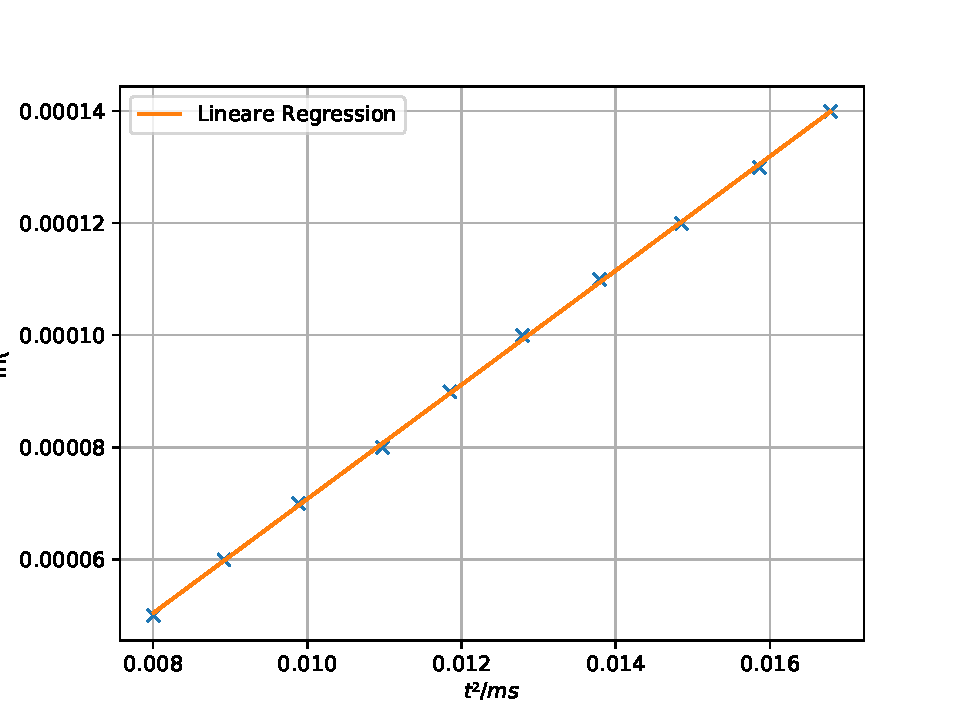
\includegraphics[width=0.45\textwidth]{Graphibitte.pdf}
%  \caption{Plot.}
%  \label{fig:plot}
%\end{figure}

%\FloatBarrier

%Einheiten: \SI{3}{\newton\s}
%1,41 \cdot \cramped{10^{-3}} ~s  für hochzahlen

%\begin{table}
%  \centering
%  \caption{Tabelle für a)Erste Bestimmung der Zeitkonstanten}
%  \label{Tab1}
%    \begin{tabular}{c c}%c zeigt die anzahl der Spalten
%      \toprule
%      Spannung $U_c$ &Zeit $t$\\% \\ werden benötigt um die Zeile zu Beenden
%      mV&ms\\% & Zeichen grenzen die Zahlen voneinander ab.
%      \midrule
%      \midrule
%        %\input{tab1.txt}% Die Tabelle ist hier ausgelagert. Sie kann aber auch genausogut hier eingefügt werden.
%          0,000 &     752\\
%          0,400 &     440\\
%          0,800 &     448\\
%      \bottomrule
%    \end{tabular}
%\end{table}

%\begin{table}
%    \centering
%    \caption{Messwerte für die Beta-Strahlung.}
%    \label{Tabg}
%    \sisetup{table-format=1.2}
%    \begin{tabular}{S S[table-format=2.2] S } %3 ziffern vom kommer, zwei danach, geht hiter jedes s
%      \toprule
%      %{$D$/cm}& \multicolumn{5}{c}{$U_{\symup{B}i} = \,\si{V}$}\\ überschrift über mehrere spalten
%      %\midrule
%       {$D/ \mu\si{m}$}& {$R/\frac{\si{kg}}{\si{m²}}$} & {$t$/s} &  {$N$} & {$A_{\symup{gem}} = \frac{N}{t}/ \frac{1}{\si{s}}$}  & {$A/ \frac{1}{\si{s}}$}  & {$\symup{ln}(A)$}\\
%      \midrule
%      \midrule
%          {$ 3924 \pm 62$} & 39,24 & {$ ~~3,652 \pm 0,016$}\\
%          {$ 2122 \pm 46$} & 10,61 & {$ ~~2,296 \pm 0,023$}\\
%          {$ 3001 \pm 54$} & 10,00 & {$ ~~2,233 \pm 0,019$}\\
%      \bottomrule
%    \end{tabular}
%\end{table}

%Mittelwert von X:
%\begin{equation*}
%  \overline{X }=  \frac{1}{N} \sum_{i=1}^N (X_i) = 75,98 \, \si{Hz} 
%\end{equation*}
%Formel für den Fehler des Mittelwerts:
%\begin{equation*}
%  \symup{\Delta} X = \frac{1}{\sqrt{N}} \sqrt{\frac{1}{\sqrt{N-1}} \sum_{i=1}^N (X_{i}-\overline{X})²}= 0,02 \, \si{Hz} 
%\end{equation*}